\chapter{Evaluation}
\label{sec:eval}

Sections \ref{sec:p1test} and \ref{sec:p2test} detail the testing process for the two development phases of the project. This section will present the results of testing and evaluate the success of the project using these results.

\section{Phase One}

\subsection{Genetic Algorithm}

\subsubsection{Test Setup}
The parameters used to test the genetic algorithm are listed below. These are discussed in section \ref{sec:gaparams}.
\begin{itemize}
  \item{Fitness function = De Jong's function 1}
  \item{$x_{min}$ = -5.12}
  \item{$x_{max}$ = 5.12}
  \item{Population size = 50}
  \item{Number of generations = 1000}
  \item{Number of chromosomes = 1}
  \item{Number of genes = 20}
  \item{Number of bits to represent each gene = 10}
  \item{Number of parents = 50}
  \item{Crossover rate = 0.6}
  \item{Mutation rate = 0.001}
\end{itemize}

\subsubsection{Binary Tournament Selection Results}
The optimisation graphs for optimising De Jong's function 1 with binary tournament selection are shown in appendix \ref{sec:appendix3} and \ref{sec:appendix4}. Looking at the graphs, it can be seen that the genetic algorithm has performed well at optimising De Jong's function 1. From the graphs, the GA locates the area containing the optimum within 200-300 generations. For maximisation, that optimum looks to be close to 525, and for minimisation, close to 0. Considering that the maximum value for De Jong's function  in the range [-5.12, 5.12] is 524.288 and the minimum 0, the genetic algorithm has converged quickly to a good optimum. The output of the genetic algorithm supports the data shown by the graph. Each iteration, the GA outputs the best value in its current population (this output has not been included for compactness). The output of the GA shows that it optimised to an optimum of 524.288 for maximisation and $5.00977\e{-4}$ for minimisation. The speed at which these optima were reached differed between one and two-point crossover. For one-point crossover, the minimum was reached in 385 generations and the maximum in 328. For two-point crossover, the minimum was reached in 318 and the maximum 321. Two-point crossover converged slightly faster, which can be explained by the fact that, in general, two-point is going to introduce less diversity into the population, as fewer bits will be exchanged between parent individuals. This will reduce how explorative the population is.

\subsubsection{Rank Selection Results}
The optimisation graphs for optimising De Jong's function 1 with rank selection are shown in appendix \ref{sec:appendix5} and \ref{sec:appendix6}. As with binary tournament selection the graphs show that the genetic algorithm has optimised De Jong's function 1 well; locating the are containing the optimum within 200-300 generations. For maximisation, that optimum looks to be close to 525, and for minimisation, close to 0, so the genetic algorithm has converged quickly to a good optimum. The output of the genetic algorithm supports the data shown by the graph; a maximum of 524.288 was reached and a minimum of $5.00977\e{-4}$ reached, these are the same maximum and minimum binary tournament found. As with binary tournament selection, the choice of one or two-point crossover affects the convergence speed of the algorithm. For one-point crossover, the minimum was reached in 314 generations and the maximum in 210 and for two-point crossover, the minimum was reached in 286 and the maximum 309.

\subsubsection{Proportional Selection Results}
The results of the proportional selection tests can be seen in appendix \ref{sec:appendix7} and \ref{sec:appendix8}. In comparison with the graphs for binary tournament and rank selection, the proportional graphs show a poorly performing algorithm. For maximisation, there is wide diversity in the population and a maximum of less than 500 has been reached. For minimisation, the graph shows the population has been maximised, which suggests the scaling method is not working effectively. After a number of experiments, it was found that the proportional selection GA implemented is greatly affected by the number of parents parameter, and therefore the number of offspring produced by crossover. By adjusting the value of this parameter, the performance of the GA can be greatly improved, as shown by appendix \ref{sec:appendix9}. For minimisation the GA is now using 10 parents and for maximisation 20. The performance of the GA now matches the performance of binary tournament and rank selection. A maximum of 524.288 has been found and a minimum of 3.30956. Whilst the accuracy has been improved, the convergence speed is still significantly worse than that of the other selection methods; maximisation took 706 generations and minimisation 881.

\subsubsection{Comparison With Shark}
For the next stage of testing, the comparison between the author's implementation and a similar implementation in the Shark machine learning library, a genetic algorithm with binary tournament selection and two-point crossover was chosen. Whilst rank selection had been shown to have slightly better performance to binary tournament selection, the author was unable to find a similar implementation of the linear ranking method in the Shark library, so binary tournament selection was chosen to ensure a fair comparison. Two-point crossover was chosen as it had resulted in slightly better performance over one-point crossover with binary tournament selection. The results of optimisation with the Shark implementation can be found in appendix \ref{sec:appendix10}. Comparing this to the graphs in appendix \ref{sec:appendix3}, the Shark implementation seems to perform similarly to the project's implementation. Looking at the actual output of the Shark implementation, the algorithm has found a minimum of $5.00977\e{-4}$ and a maximum of 524.288, which are the same as those found by the project's implementation. The convergence speeds are also similar, with the Shark implementation taking 310 and 324 generations for minimisation and maximisation. 

\subsubsection{Evaluation}
The genetic algorithm has been implemented successfully to a strong degree. In accordance with the requirements of the system (section \ref{sec:require}), the genetic algorithm has been implemented supporting a number of selection and recombination modes, and the modes to be used, as well as the other configurable parameters, can be easily changed through the algorithm's constructor. The majority of the supported selection modes perform very well, with similar accuracy and convergence speed as a similar implementation in the Shark machine learning library. The proportional selection mode is the exception, as it performs very badly. However, through careful parameter tuning, proportional selection can be made to perform significantly better, but still worse than the other selection modes. The algorithm is able to optimise De Jong's function 1 very well, actually reaching the maximum value and finding a very small minimum: $5.00977\e{-4}$. The algorithm is unable to minimise any lower than $5.00977\e{-4}$ because at that point, the value of the genes are as small as they can be given the number of bits used to represent them. Because of how the decoding equation works, the genes are only able to take certain values, determined by the bounds of the function and the number of bits that represent each gene. By increasing the number of bits, the precision of the genes would be increased, and therefore smaller minima could be found.

\subsection{Evolution Strategies}

\subsubsection{Test Setup}
The test setup for the evolution strategies algorithm is discussed in section \ref{sec:esparams}, it is listed again here for ease of reference.
\begin{itemize}
  \item{Fitness function = De Jong's function 1}
  \item{$x_{min}$ = -5.12}
  \item{$x_{max}$ = 5.12}
  \item{Population size = 50}
  \item{Number of generations = 1000}
  \item{Number of chromosomes = 2}
  \item{Number of genes = 20}
  \item{Number of strategy parameters = 1}
  \item{Number of parents per offspring = 2}
  \item{Number of offspring = 50 or100}
\end{itemize}

\subsubsection{$(\mu,\lambda)$ Selection Results}
The graphs in appendix \ref{sec:appendix11}, \ref{sec:appendix12}, \ref{sec:appendix13} and \ref{sec:appendix14} show the results of optimising De Jong's function 1 using a $(\mu,\lambda)$ evolution strategy algorithm. Looking at the graphs it is clear that the convergence speed of $(\mu,\lambda)$ ES is better than that of GAs; the area containing the optimum is reached within 100-200 generations. It is also clear that the performance of intermediate recombination is completely undefined for maximisation problems in this implementation. Looking at the output of the algorithm, when minimising very small minima are found. For discrete and global discrete recombination, minima of $3.7767\e{-21}$ and $5.7056\e{-14}$ were found and for intermediate and global intermediate, minima of $3.6096\e{-44}$ and $9.2004\e{-41}$. After the 1000 generations, the minimum was still decreasing so if more generations were produced the minima found by the algorithm would get even smaller, and may eventually reach the true minimum of 0. For maximisation, the maximum value of 524.288 was reached by both discrete and global discrete recombination, with a convergence speed of 289 and 233 generations respectively.

\subsubsection{$(\mu+\lambda)$ Selection Results}
Appendix \ref{sec:appendix15}, \ref{sec:appendix16}, \ref{sec:appendix17} and \ref{sec:appendix18} show the results of optimising using the $(\mu+\lambda)$ evolution strategy algorithm. The performance of $(\mu+\lambda)$ is very similar to that of $(\mu,\lambda)$. The area containing the optimum is located within 100-200 generations and intermediate and global intermediate recombination still performs badly for maximisation; the diversity is lesser, but the true maximum is still not found. Again, very small minima are found; $6.535\e{-41}$, $1.2289\e{-38}$, $1.4018\e{-43}$ and $1.8098\e{-42}$ for discrete, global discrete, intermediate and global intermediate recombination, and as with $(\mu,\lambda)$, if the number of generations were increased, smaller minima would be found. For maximisation, discrete and global discrete recombination both reach 524.288, requiring 345 and 289 generations to do so.

\subsubsection{Comparison with Shark}
For the comparison with the Shark implementation, a $(\mu+\lambda)$ ES with discrete recombination was chosen. $(\mu+\lambda)$ selection was chosen, because whilst its convergence speed was slightly slower that $(\mu,\lambda)$, it requires the generation of less offspring which makes the production of each generation more efficient. Discrete recombination was chosen because it was one of the two recombination modes that worked for both minimisation and maximisation. It was chosen over global discrete recombination because the Shark library does not provide a method to perform global recombination by default. The results of optimisation using the Shark implementation can be seen in appendix \ref{sec:appendix19}. The performance of the Shark implementation and the project's are vary similar. For minimisation, both identify the area containing the optimum within 100-200 generations and reach very low minima, the Shark implementation reaching $3.91939\e{-17}$. Both implementations would also find smaller minima if the number of generations was increased. For maximisation, the same is true, the area containing the maximum is found with 100-200 generations and then the maximum of 524.288 reached within another 100 generations or so, the Shark implementation taking 309 generations in total.

\subsubsection{Evaluation}
The evolution strategies algorithm has been implemented effectively but with some problems. As per the project requirements (section \ref{sec:require}), a number of different selection and recombination modes are supported and these, along with the other configurable parameters, can be easily changed through the algorithm's constructor. The algorithm is able to optimise De Jong's function 1 extremely well, finding the maximum of 524.288 and finding very small minima. This shows that another system requirement has been met; the algorithm has not explored outside the bounds of the function, showing that the constraint handling mechanism works successfully. It is still able to find values on the bounds of the search space too, again showing that the constraint handling method is effective. Unlike the genetic algorithm, where the accuracy of the minimum is limited by the number of bits used to represent each gene, because ES use real value coding there is no limit on how small the values of the genes can become; the only limiting factor to the minimum identified by the algorithm is the number of generations. Not only is the accuracy of the ES algorithm good, but the convergence speed is fast too, typically identifying the area containing the optimum in 100-200 generations and then identifying the optimum in less than 350. The implementation of ES also matches the performance of a Shark implementation very closely. The limitation with this ES implementation is that the performance of intermediate and global intermediate recombination is undefined for maximisation problems.

\subsection{Particle Swarm Optimisation}

\subsubsection{Test Setup}
The test setup for particle swarm optimisation is discussed in section \ref{sec:psoparams}, it is listed again here for ease of reference.
\begin{itemize}
  \item{Fitness function = De Jong's function 1}
  \item{$x_{min}$ = -5.12}
  \item{$x_{max}$ = 5.12}
  \item{Population size = 50}
  \item{Number of generations = 1000}
  \item{Number of chromosomes = 2}
  \item{Number of genes = 20}
  \item{Number of velocities = 20}
  \item{Velocity clamping factor = 0.25}
\end{itemize}

\subsubsection{Optimisation Results}
Appendix \ref{sec:appendix20} shows the optimisation graphs for the particle swarm optimisation algorithm. The graphs show a wide diversity in the population during the first 100-200 generations before the diversity steadily decreases as the population moves towards the optimum. This sort of pattern is expected, as the particles are initially distributed evenly in the search space and slowly move towards the best value found so far. When maximising De Jong's function 1, the population split into two branches; one converging on the optimum and the other remaining between 75 and 200. This suggests that PSO may have problems solving more complex maximisation problems. The accuracy of the algorithm is good, reaching the maximum of 524.288 and a minimum of $3.8202\e{-10}$. As with evolution strategies, the accuracy of the minimum value is limited by the number of generations; if the number of generations were increased then smaller minima could be found. The graphs clearly show that the convergence speed of PSO is much slower than that of genetic algorithms or evolution strategies, with maximisation taking 929 generations to reach the maximum. This is to be expected however, because of the way in which the algorithm works.

\subsubsection{Comparison With Shark}
Appendix \ref{sec:appendix21} shows the optimisation results of a PSO implemented in Shark. The performance of the Shark implementation is almost identical to the implementation in this project. A similar pattern if produced in the graphs, with the population starting off diverse and then steadily converging, and the population splitting into two branches when solving a maximisation problem. The accuracy of the two implementations are similar, both reaching the maximum 524.288, and the Shark implementation reaching a minimum of $3.89969\e{-8}$, again limited by the number of generations. The convergence speed is near identical as well, with the Shark implementation taking ever so slightly less generations to reach the maximum, 921 as opposed to 929.

\subsubsection{Evaluation}
The implementation of particle swarm optimisation is highly effective. Both maximisation and minimisation problems are solved with the same accuracy as that of the genetic and evolution strategies algorithms and the implementation matches very closely the equivalent in Shark. Again, minimisation accuracy is limited only by the number of generations, giving PSO an advantage over GAs for minimisation. The convergence speed is significantly slower when compared with GAs or ES, but this is to be expected given the operation of the PSO algorithm. The only limitation is that when maximising the population split into two branches, one of which does not converge. This suggest that the algorithm could have problems optimising more complex maximisation problems.

\subsection{Evaluation of Phase One}
One of the objectives of this project was to "Implement and test the chosen population based optimisation algorithms, producing a generic implementation". The algorithms chosen were the genetic, evolutions strategies and particle swarm optimisation algorithms and the results of testing these algorithms with De Jong's function 1 are presented and discussed above. The results show that the three algorithms have been successfully implemented and perform well at optimising arbitrary maximisation or minimisation problems. In accordance with the requirements of the project, a number of selection and recombination modes are supported, the majority of which perform extremely well. Some of these modes do not work as expected; proportional selection and intermediate recombination, and this limits the success of the optimisation library slightly. The optimisation library developed in phase 1 also meets many of the other project requirements; the algorithms optimise only within the bounds of the problem, the optimisation results can be plotted to a scatter graph once optimisation is finished, the algorithms can be easily configured through their constructors and new problems, algorithms and stopping criteria can be easily added by overriding a few methods in the class hierarchy. In general, the system produced in phase one meets the project objective and requirements to a strong extent, limited only by the fact that a small number of the selection and recombination modes do not work as intended.
\\\\Another objective of the project was to "Compare the effectiveness and efficiency of the different algorithms". The test results obtained show a number of differences between the different algorithms. 
\\With regards to efficiency, or convergence speed, the results show that evolution strategies is the fastest algorithm, generally finding the area containing the optimum in 100-200 generations and finding the optimum in less than 350. The genetic algorithm is the next fastest, taking only slightly longer than evolution strategies. The slowest algorithm by far is particle swarm optimisation, taking over 900 generations to find the optimum. This is to be expected though, considering the operation of the particle swarm optimisation algorithm. 
\\Regarding effectiveness, or accuracy, for maximisation the results obtained show that all the algorithms have the same accuracy, all of them identifying the true maximum value of 524.288. For minimisation however, the genetic algorithm was shown to have the lowest accuracy, only finding a value of $5.00977\e{-4}$. This however is the smallest value the algorithm could find given a 10 bit representation per gene; if the number of bits per gene were increased then smaller minima could be found. As for the accuracy of evolution strategies and particle swarm optimisation, they were more accurate than the genetic algorithm, and their accuracy was limited by the number of generation produced. When 1000 generations were reached, both of the algorithms were still finding smaller and smaller minima; if the number of generations were increased, even smaller values would be found, and the true minimum of 0 may even be reached.

\section{Phase Two}

\subsection{Genetic Algorithm}

\subsubsection{Test Setup}
The parameters used for testing the genetic algorithm are listed below
\begin{itemize}
  \item{Fitness function = function \ref{eq:connect4}}
  \item{$x_{min}$ = 0}
  \item{$x_{max}$ = 1}
  \item{Population size = 10}
  \item{Number of generations = 1000}
  \item{Number of chromosomes = 3}
  \item{Number of genes = 4, 4, 7}
  \item{Number of bits to represent each gene = 10}
  \item{Selection mode = binary tournament}
  \item{Number of parents = 10}
  \item{Crossover mode = two-point}
  \item{Crossover rate = 0.6}
  \item{Number of parents per generation = 10}
  \item{Mutation rate = 0.001}
\end{itemize}

\subsubsection{Testing Results}
Table \ref{tab:game} shows the results of the 50 games the genetic algorithm played against the author. It is clear from these results that the genetic algorithm is not playing Connect 4 especially well. It plays slightly better when playing as player1, but was still not capable of beating the author. The majority of the games were very short, typically finishing within 20 moves. Whilst playing the algorithm, the author noticed several problems with the way it was playing. The first, and most critical, was that the genetic algorithm played in patterns; that is, if the author played counters in certain places then the algorithm would always play the same counters in the same order. This made the algorithm very exploitable and therefore, it was extremely easy for the author to win. This pattern was mostly noticeable when the genetic algorithm was player2. A second defect the author noticed was that the algorithm would not always complete its three in a rows, or block the author's. This shows that the algorithm has not learnt the game effectively, as the probability to finish a three in a row, whether the opponents or yours, should be 1.
\begin{table}[tp]
   \begin{minipage}{\textwidth}
      \begin{center}
         \begin{tabular}{c|c|c|c}
           & Genetic Algorithm Wins & Author Wins & Draws\\
           \hline
           GA player1 & 6 & 18 & 1 \\
           GA player2 & 0 & 25 & 0
         \end{tabular}
      \end{center}
   \end{minipage}
   \caption{Genetic algorithm Connect 4 results against the author}
   \label{tab:game}
\end{table}
\begin{table}[tp]
   \begin{minipage}{\textwidth}
      \begin{center}
         \begin{tabular}{c|c|c|c}
           Time Limit & Genetic Algorithm Wins & Recursive Wins & Draws\\
           \hline
           5 seconds & 3 & 994 & 3 \\
           1 second & 12 & 972 & 16 \\
           0.5 seconds & 10 & 963 & 27 \\
           0.25 seconds & 13 & 968 & 19 \\
           0.15 seconds & 35 & 930 & 35
         \end{tabular}
      \end{center}
   \end{minipage}
   \caption{Genetic algorithm Connect 4 results against the recursive module}
   \label{tab:gare}
\end{table}
\begin{figure}[tp]
   \begin{center}
     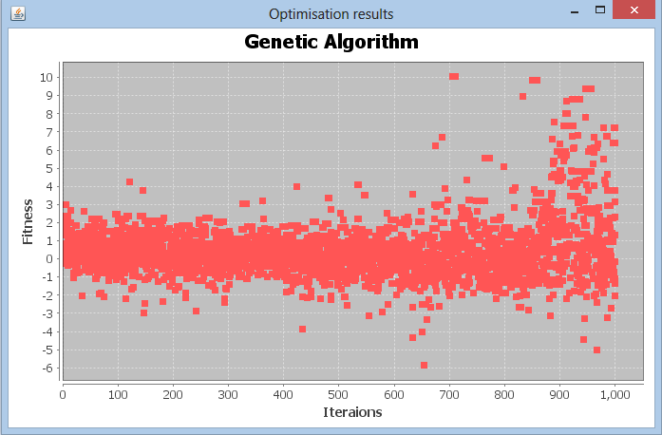
\includegraphics{Figures/gaconnect4}
   \end{center}
   \caption{Genetic algorithm optimisation results for Connect 4}
   \label{fig:gaconnect4}
\end{figure} 
\\The results of the 1000 games against the recursive module (table \ref{tab:gare}) also show a poor playing performance by the genetic algorithm. The playing performance increases as the turn time decreases, which was expected, but the algorithm was not able to evenly closely match the performance of the recursive module. At a time limit of 0.15 seconds, the algorithm's performance was significantly higher than the others which suggests that at even smaller time limits the algorithm may be able to match, or even out perform, the recursive module. Unfortunately, it is not possible to test smaller time limits, as below 0.15 seconds the genetic algorithm exceeds the time limit and the recursive player wins by default.
\\Looking at the optimisation results of the genetic algorithm, shown in figure \ref{fig:gaconnect4}, it is clear that the population has not been optimised at all, which explains why the playing performance is poor.

\subsection{Evolution Strategies}

\subsubsection{Test Setup}
The parameters used for testing evolution strategies are listed below
\begin{itemize}
  \item{Fitness function = function \ref{eq:connect4}}
  \item{$x_{min}$ = 0}
  \item{$x_{max}$ = 1}
  \item{Population size = 10}
  \item{Number of generations = 1000}
  \item{Number of chromosomes = 4}
  \item{Number of genes = 4, 4, 7}
  \item{Number of strategy parameters = 1}
  \item{Selection mode = $(\mu+\lambda)$}
  \item{Recombination mode = Discrete recombination}
  \item{Number of parents per offspring = 5}
  \item{Number of offspring = 10}
\end{itemize}

\subsubsection{Testing Results}
Table \ref{tab:esme} shows the results of the 50 games  played by the evolution strategies algorithm against the author. From these results, it can be seen that the evolution strategies algorithm has learnt to play Connect 4 better than the genetic algorithm. The algorithm plays best when it is player1, actually beating the author over the 25 games. Whilst playing the algorithm, the author noticed several things. Firstly, that the games were significantly longer than those against the genetic algorithm, often nearly filling the entire board. Secondly, that the algorithm was capable of setting traps to guarantee that it won; i.e. playing so that the author had to play two counters in the same row to prevent it from winning or forcing the author to block in one column which enabled the algorithm to win next turn. Both of these features suggest that the algorithm has learnt to play Connect4 to a good extent. There were however still some problems the author noticed; the algorithm still occasionally played in patterns which could be exploited and occasionally didn't block the author's three in a rows. Both of these limitations show that the algorithm has not completely learnt to play Connect 4.
\begin{table}[tp]
   \begin{minipage}{\textwidth}
      \begin{center}
         \begin{tabular}{c|c|c|c}
           & Evolution Strategy Wins & Author Wins & Draws\\
           \hline
           ES player1 & 15 & 10 & 0 \\
           ES player2 & 6 & 19 & 0
         \end{tabular}
      \end{center}
   \end{minipage}
   \caption{Evolution strategies Connect 4 results against the author}
   \label{tab:esme}
\end{table}
\begin{table}[tp]
   \begin{minipage}{\textwidth}
      \begin{center}
         \begin{tabular}{c|c|c|c}
           Time Limit & Evolution Strategy Wins & Recursive Wins & Draws\\
           \hline
           5 seconds & 0 & 999 & 1 \\
           1 second & 3 & 993 & 4 \\
           0.5 seconds & 11 & 987 & 2 \\
           0.25 seconds & 28 & 966 & 6 \\
           0.15 seconds & 40 & 947 & 13
         \end{tabular}
      \end{center}
   \end{minipage}
   \caption{Evolution strategies Connect 4 results against the recursive module}
   \label{tab:esre}
\end{table}
\begin{figure}[tp]
   \begin{center}
     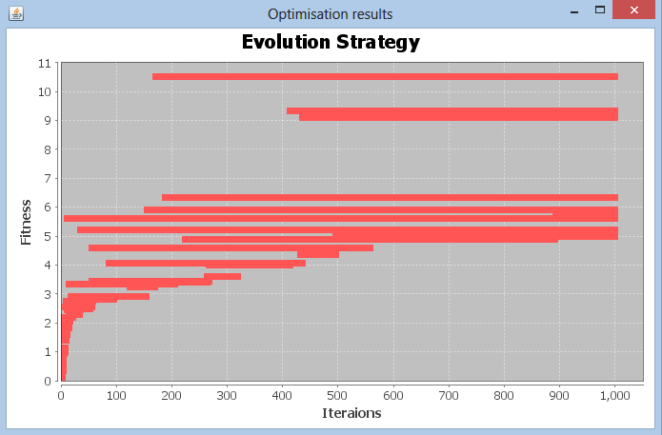
\includegraphics{Figures/esconnect4}
   \end{center}
   \caption{Evolution strategies optimisation results for Connect 4}
   \label{fig:esconnect4}
\end{figure} 
\\The results of the 1000 games against the recursive module (table \ref{tab:esre}) show a slightly different story. The playing performance still increases as the turn time decreases, as expected, but overall the performance is worse than that of the genetic algorithm. ES wins more games than the genetic algorithm, but overall the recursive module wins more when playing against the ES algorithm. The optimisation results, shown in figure \ref{fig:esconnect4}, could help explain this, as they show that some maximisation has taken place in the population. This means that the algorithm has learnt the playing algorithm to an extent and therefore will play less randomly. This lack of randomness may be the reason why evolution strategies performs worse against the recursive module than the genetic algorithm, as the random aspect of the GA may be harder for the recursive module to predict. As with the genetic algorithm results, performance significantly increases at 0.15 seconds but it is not possible to test lower time limits, since the algorithm will exceed the time limit.

\subsection{Particle Swarm Optimisation}

\subsubsection{Test Setup}
The parameters used for testing particle swarm optimisation are listed below
\begin{itemize}
  \item{Fitness function = function \ref{eq:connect4}}
  \item{$x_{min}$ = 0}
  \item{$x_{max}$ = 1}
  \item{Population size = 10}
  \item{Number of generations = 1000}
  \item{Number of chromosomes = 4}
  \item{Number of genes = 4, 4, 7}
  \item{Number of velocities = 7}
  \item{Velocity clamping factor = 0.25}
\end{itemize}

\subsubsection{Testing Results}
The results of the 50 games particle swarm optimisation played against the author are shown in table \ref{tab:psome}. From these results, it can be seen that particle swarm optimisation plays slightly better than the genetic algorithm, able to win games against the author when player2, but not as well as evolution strategies. As with evolution strategies, the games against this algorithm were long, and it exhibited some ability to set traps, both of which suggest a good level of learning. However, the algorithm still did not always block the author so it cannot have learnt to play Connect 4 fully. 
\begin{table}[tp]
   \begin{minipage}{\textwidth}
      \begin{center}
         \begin{tabular}{c|c|c|c}
           & Particle Swarm Optimisation Wins & Author Wins & Draws\\
           \hline
           PSO player1 & 7 & 18 & 0 \\
           PSO player2 & 7 & 18 & 0
         \end{tabular}
      \end{center}
   \end{minipage}
   \caption{Particle swarm optimisation Connect 4 results against the author}
   \label{tab:psome}
\end{table}
\begin{table}[tp]
   \begin{minipage}{\textwidth}
      \begin{center}
         \begin{tabular}{c|c|c|c}
           Time Limit & Particle Swarm Optimisation Wins & Recursive Wins & Draws\\
           \hline
           5 seconds & 1 & 995 & 4 \\
           1 second & 2 & 997 & 1 \\
           0.5 seconds & 11 & 985 & 4 \\
           0.25 seconds & 10 & 986 & 4 \\
           0.15 seconds & 17 & 980 & 3
         \end{tabular}
      \end{center}
   \end{minipage}
   \caption{Particle swarm optimisation Connect 4 results against the recursive module}
   \label{tab:psore}
\end{table}
\begin{figure}[tp]
   \begin{center}
     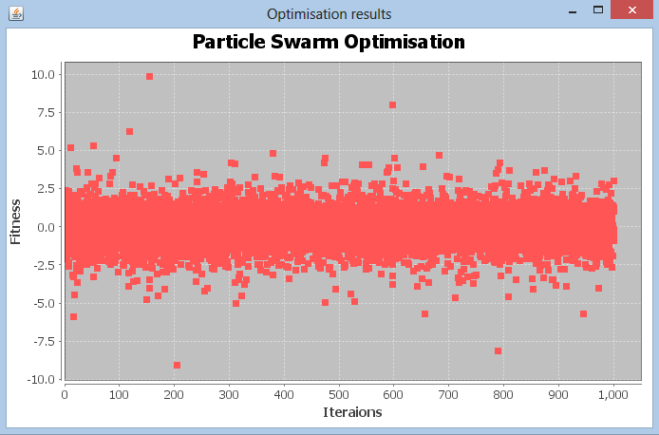
\includegraphics{Figures/psoconnect4}
   \end{center}
   \caption{Particle swarm optimisation optimisation results for Connect 4}
   \label{fig:psoconnect4}
\end{figure} 
\\The results of the 1000 games against the recursive module (table \ref{tab:psore}) show a poor performance too. As with the other two algorithms, performance increases as the turn time decreases but the performance of particle swarm optimisation is the worse of any of the three algorithms. The optimisation results of particle swarm optimisation, figure \ref{fig:psoconnect4}, are similar to that of the genetic algorithm, except clustered around an even smaller area. This not only shows that the population has not been optimised but also that there has been only weak exploration, which could explain why the algorithm performed worse than the genetic algorithm, as there will be less randomness in the population.

\subsection{Evaluation of Phase Two}
The two project objectives the second phase of this project aimed to achieve were "Adapt the generic implementation to work with Connect 4 in The Arena" and "Evaluate the effectiveness of the different algorithms in playing Connect 4". With regards to the first objective, this has been achieved strongly, as all three algorithms are capable of playing Connect 4 in The Arena and performing optimisation using Connect 4 as a fitness function. The effectiveness of this optimisation and how the algorithms play Connect 4 is questionable however. 
\\When playing against the author, evolution strategies is the strongest algorithm, especially when player1, actually beating the author. The genetic algorithm is clearly the worst algorithm, incapable of winning any games when player2 and only winning 6 when player1, and particle swarm optimisation performs only slightly better. The optimisation graphs for the algorithms support this as they show that evolution strategies was the only algorithm to undergo any form on optimisation, even if that optimisation is extremely limited. The graphs for particle swarm optimisation and the genetic algorithm are very similar, both showing a wide diversity and no optimisation, hence why they performed similarly against the author.
\\The results of the tests to match the playing performance of the recursive player show that none of the algorithms were able to even closely match the performance of the recursive player. Again, evolution strategies won the most games but overall the genetic algorithm plays best against the recursive player; with more wins and draws more than any other algorithm. The particle swarm optimisation algorithm is the worst performing. Looking at the optimisation graphs, the results suggest that the randomness the genetic algorithm has due to poor optimisation works better against the recursive player than the rules evolution strategies has learnt. The performance of each algorithm increased as the turn limit was decreased, which was expected as it limits the effectiveness of the recursive player, and increased significantly at 0.15 seconds for the evolution strategies and genetic algorithms. This suggests that at even lower turn limits, these algorithms may be able to match, or even exceed, the recursive player. Unfortunately it is not possible to test any smaller time limits, as the algorithms start to exceed smaller time limits than 0.15 seconds and the recursive player wins by default.